\section{Implementierung}

In diesem Kapitel wird die Umsetzung des Projektes mit Fokussierung auf die einzelnen Komponenten, sowie die Kommunikation beschrieben.

\subsection{Kommunikation}

\begin{figure}[h]
	\begin{center}
		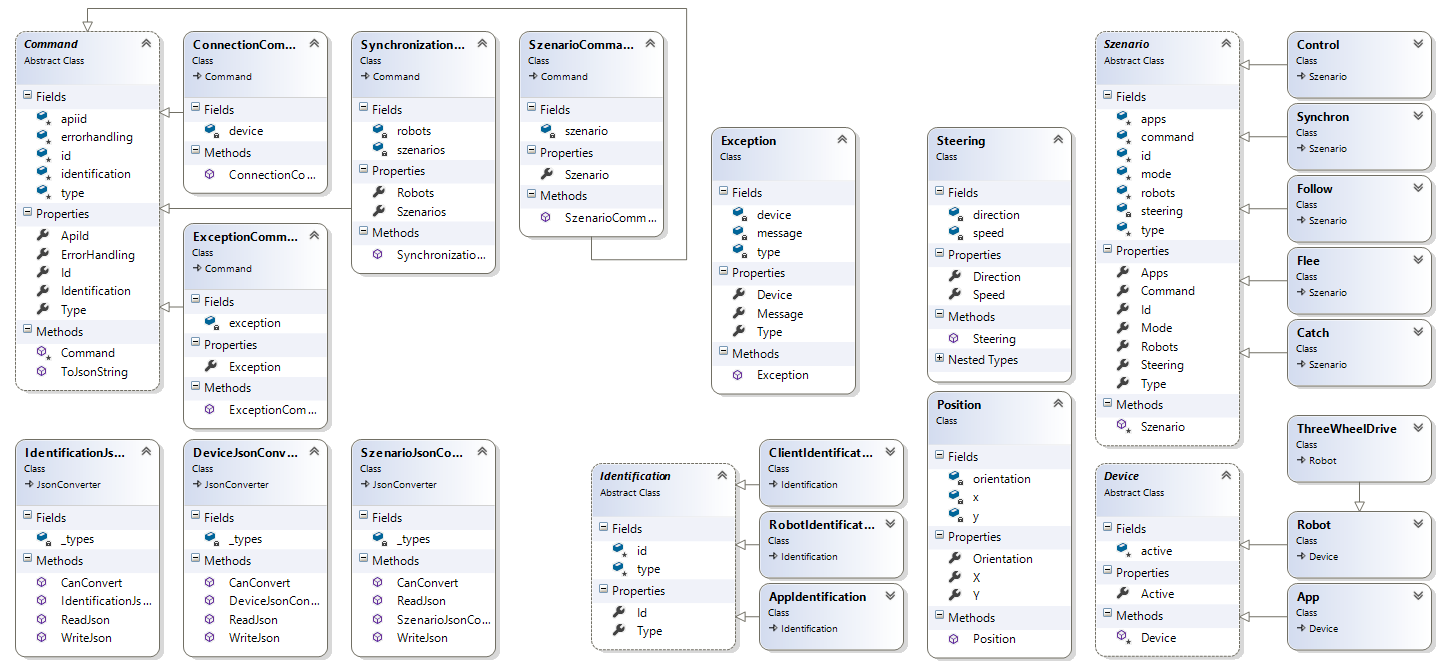
\includegraphics[width=0.95\textwidth]{images/uml/full_class_diagram.png}
	\end{center}
	\caption{Aufbau Commands}
	\label{fig:full_classdiagram}
\end{figure}

\begin{figure}[h]
	\begin{center}
		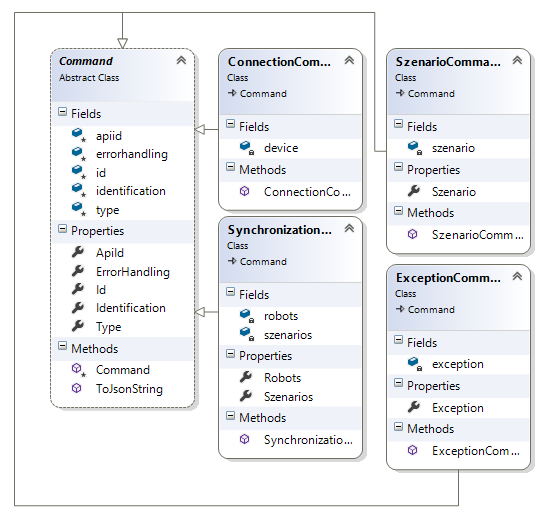
\includegraphics[width=0.95\textwidth]{images/uml/commands.png}
	\end{center}
	\caption{Commands}
	\label{fig:commands_classdiagram}
\end{figure}

\begin{figure}[h]
	\begin{center}
		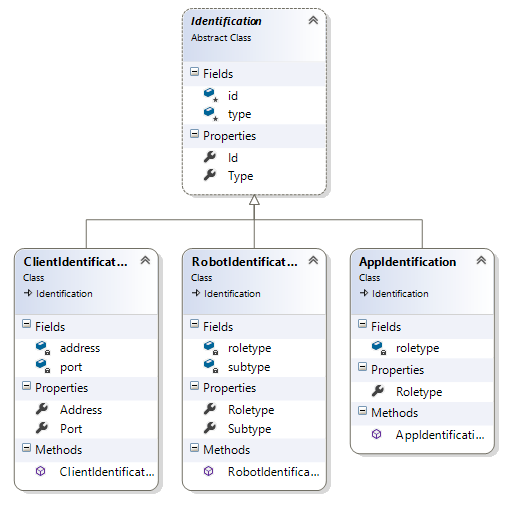
\includegraphics[width=0.95\textwidth]{images/uml/identification.png}
	\end{center}
	\caption{Identifications}
	\label{fig:identification_classdiagram}
\end{figure}

\begin{figure}[h]
	\begin{center}
		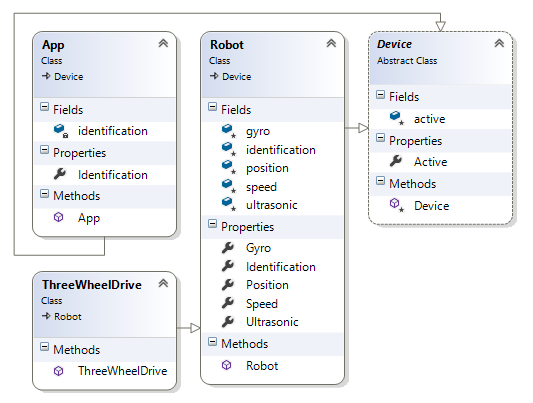
\includegraphics[width=0.95\textwidth]{images/uml/devices.png}
	\end{center}
	\caption{Devices}
	\label{fig:devices_classdiagram}
\end{figure}

\begin{figure}[h]
	\begin{center}
		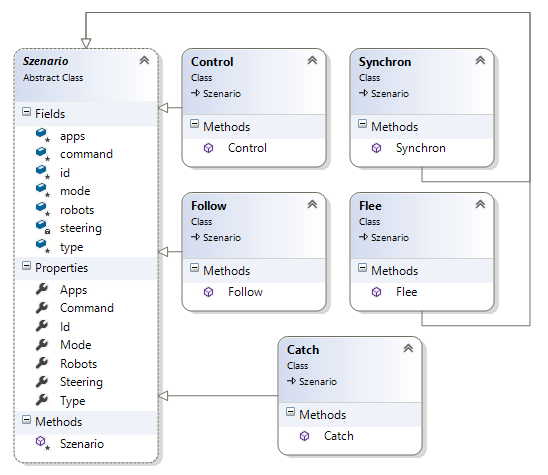
\includegraphics[width=0.95\textwidth]{images/uml/szenarios.png}
	\end{center}
	\caption{Scenarios}
	\label{fig:szenarios_classdiagram}
\end{figure}

\begin{figure}[h]
	\begin{center}
		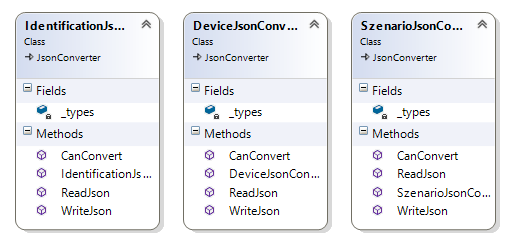
\includegraphics[width=0.95\textwidth]{images/uml/json_converter.png}
	\end{center}
	\caption{JSON Converter}
	\label{fig:converter_classdiagram}
\end{figure}

\begin{comment}
Client
Server
Interpreter
Commandostruktur
\end{comment}

\subsection{App}

\begin{comment}
Aufbau
MVVM
Binding
GUI
Library
PageModel
\end{comment}

\subsection{Backend}

\begin{comment}
Aufbau
Interpreter
Mechanismen
GUI
\end{comment}

\subsection{Robot}

\begin{comment}
Aufbau
Robot
RobotController
EV3 Library
GUI
\end{comment}